\documentclass[tikz,border=8pt]{standalone}
\usepackage{tikz}
\usepackage{xcolor}
\usetikzlibrary{arrows.meta}
\begin{document}
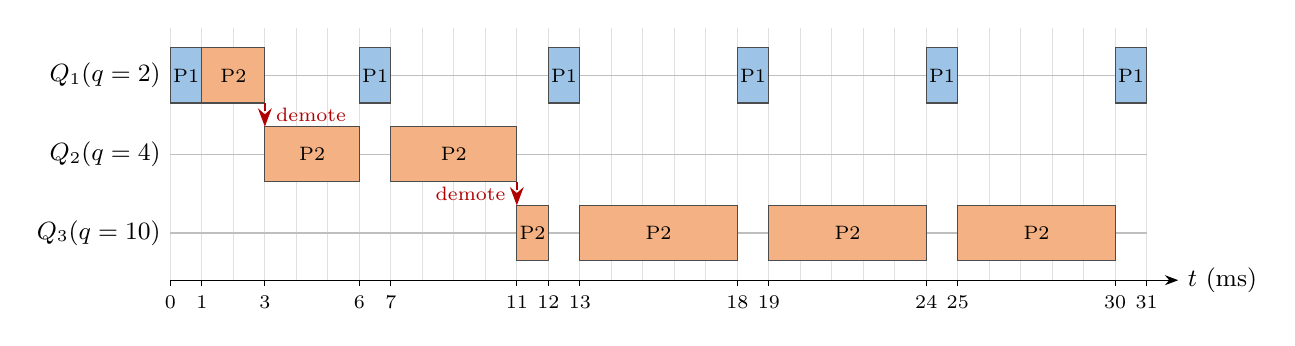
\begin{tikzpicture}[x=0.4cm,y=1cm,font=\small]

    \definecolor{pone}{RGB}{91,155,213}
    \definecolor{ptwo}{RGB}{237,125,49}

    \newcommand{\seg}[5]{%
        \draw[fill=#4!60,draw=black!70] (#1,#3-0.35) rectangle (#2,#3+0.35);
        \node[font=\scriptsize] at ({(#1+#2)/2},#3) {#5};
    }

    \foreach \x in {0,...,31}
    \draw[black!12] (\x,-0.6) -- (\x,2.6);
    \foreach \y/\q in {2/Q_1(q=2),1/Q_2(q=4),0/Q_3(q=10)}{
            \draw[black!25] (0,\y) -- (31,\y);
            \node[left] at (0,\y) {$\q$};
        }

    \draw[-{Stealth}] (0,-0.6) -- (32,-0.6) node[right] {$t$ (ms)};
    \foreach \x in {0,1,3,6,7,11,12,13,18,19,24,25,30,31}{
            \draw (\x,-0.6) -- (\x,-0.68);
            \node[below,font=\scriptsize] at (\x,-0.68) {\x};
        }

    \seg{0}{1}{2}{pone}{P1}
    \seg{6}{7}{2}{pone}{P1}
    \seg{12}{13}{2}{pone}{P1}
    \seg{18}{19}{2}{pone}{P1}
    \seg{24}{25}{2}{pone}{P1}
    \seg{30}{31}{2}{pone}{P1}

    \seg{1}{3}{2}{ptwo}{P2}
    \seg{3}{6}{1}{ptwo}{P2}
    \seg{7}{11}{1}{ptwo}{P2}
    \seg{11}{12}{0}{ptwo}{P2}
    \seg{13}{18}{0}{ptwo}{P2}
    \seg{19}{24}{0}{ptwo}{P2}
    \seg{25}{30}{0}{ptwo}{P2}

    \draw[-{Stealth},dashed,red!70!black,thick] (3,1.65) -- (3,1.35);
    \node[red!70!black,font=\scriptsize,right] at (3.05,1.5) {demote};
    \draw[-{Stealth},dashed,red!70!black,thick] (11,0.65) -- (11,0.35);
    \node[red!70!black,font=\scriptsize,left] at (10.95,0.5) {demote};

\end{tikzpicture}
\end{document}
